Ridesharing can be formulated as a decision problem where the objective is to
determine the optimal customer-to-vehicle assignments. Optimizing a single
assignment produces a \emph{local optima} whereas optimizing the aggregated
objective over all assigments in the span of a ridesharing scenario produces
the \emph{global optima}. The global optima answers questions that are of
interest to various stakeholders, such as what is the minimum fleet size needed
for an $n$\% assignment rate or what is the maximum profit achievable in a day.

To evaluate the \emph{quality} of a ridesharing algorithm (some might say the
\emph{quality of the solution} produced by the algorithm) is to measure the
value of the objective that the algorithm can achieve over the ridesharing
scenario. A high-quality algorithm achieves near the global optima whereas a
low-quality algorithm does not.  Quality of a ridesharing algorithm is
difficult to evaluate for three reasons.
\begin{enumerate}
\item \hi{Assignment Dependence.} Assignments are not independent of each
other. If a vehicle is initially assigned to a particular customer, it may be
ineligible for some future customer due to capacity and time window
constraints. This dependence means that assignments cannot be evaluated
sequentially in isolation but must be evaluated as part of a broader system.
\item \hi{Stochastic Processes.} Stochastic processes become important over the
span of a scenario.  Travel times in the road network are uncertain due to
traffic and vehicle breakdowns. Travel routes are also uncertain, if the
vehicles are non-autonomous, because human drivers can make mistakes.  If a
vehicle is initially assigned to a customer in an area that is susceptible to
traffic or difficult to navigate, it may be ineligible for some future customer
due to time window constraints. These processes cannot be ignored because they
can affect the downstream assignments.
\item \hi{Real-Time Requests.} A ridesharing algorithm's processing time
affects downstream assignments due to the real-time nature of ridesharing
requests. As a simple example, consider an algorithm that processes requests at
a rate slower than they appear. Over time, later requests may never get
processed even if valid assignments exist for them.
\end{enumerate}

The above items are all features of ridesharing in the real world.  Thus to
evaluate quality, ridesharing algorithms can be tested on actual vehicles and
customers (Figure~\ref{fig:physical}), but this method is expensive, slow to
deploy, and out of reach for most researchers. Controlled studies to determine
the effect of certain parameters, such as presence and absence of traffic, on
algorithm quality are also difficult or impossible to perform. In contrast,
testing algorithms on a simulated environment is inexpensive, fast to deploy,
readily accessible, and controllable. The challenge then becomes to design an
environment that can faithfully reproduce these real-world features. As there
is no ``lag'' in the real world, the environment must also be highly
responsive.

\begin{figure}[h]
\centering
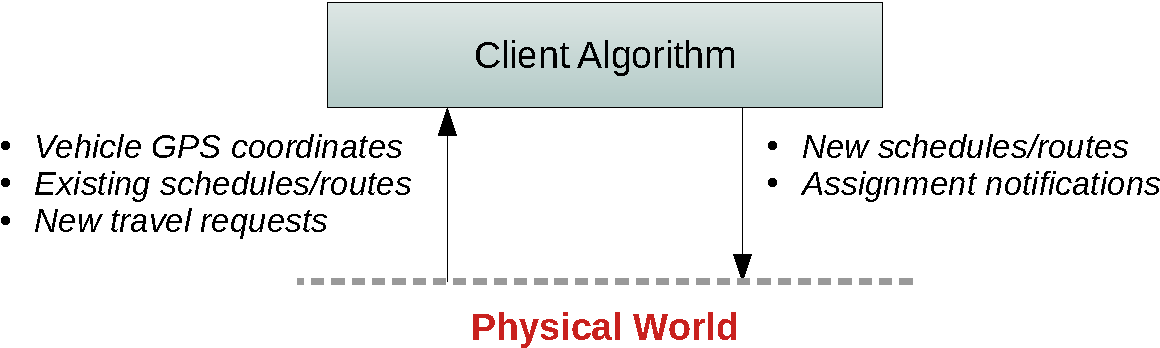
\includegraphics[width=100mm]{src/fig/physical}
\caption{To evaluate quality, ridesharing algorithms can be tested on physical
vehicles and customers, but this method is expensive, slow to deploy, and out
of reach for most researchers.}
\label{fig:physical}
\end{figure}

Jargo is the name of our environment for evaluating the quality of ridesharing
algorithms (Figure~\ref{fig:architecture}). It captures assignment dependence by
simulating real-time motion of vehicles and capacity, and it simulates
stochastic processes by perturbing route segment durations and locations. To
simulate real-time, it executes a ridesharing algorithm in parallel alongside
new requests so that an algorithm can be running while requests are arriving.
This chapter explains how Jargo's simulation data is organized, beginning with
a description of physical ridesharing (\S\ref{ch:1:sec:ridesharing-systems}), then
the mathematical model to describe physical ridesharing
(\S\ref{ch:1:sec:ridesharing-formulation}), and finally the SQL schema to store the
state data (\S\ref{ch:1:sec:ridesharing-data-model}).

\begin{figure}[h]
\centering
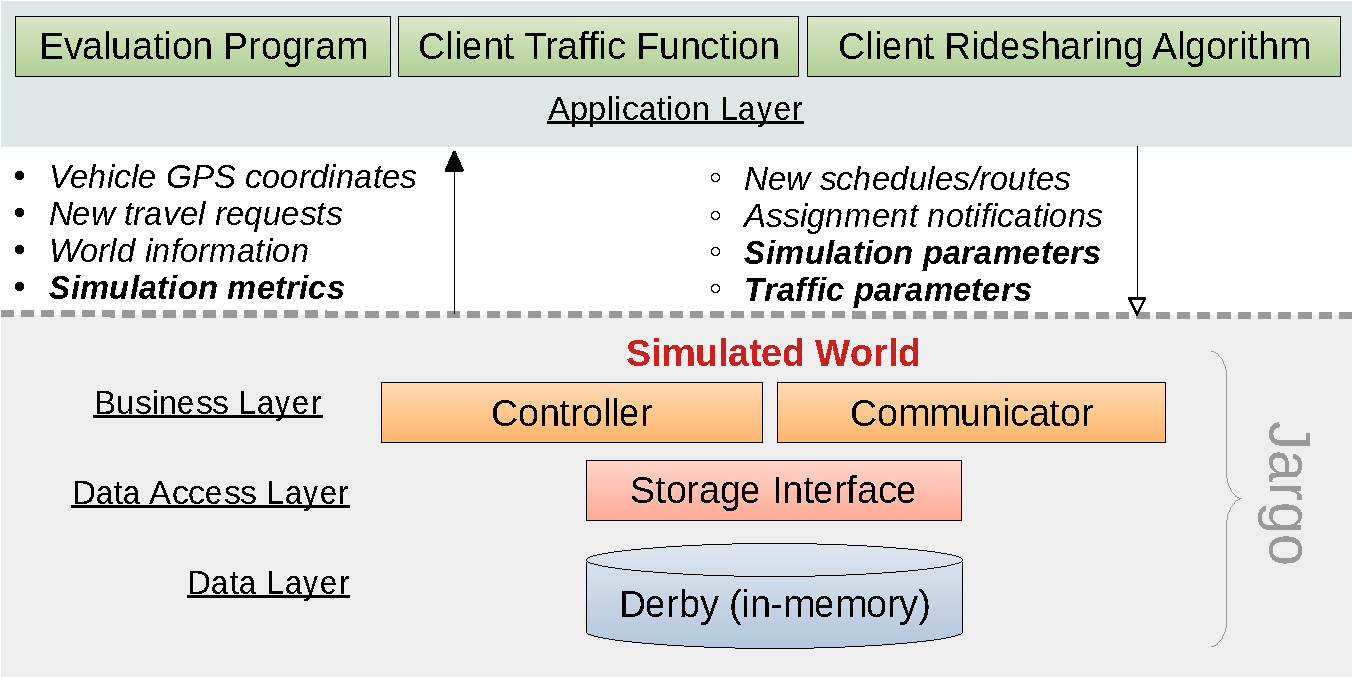
\includegraphics[width=120mm]{src/fig/architecture}
\caption{Alternatively, ridesharing algorithms can be evaluated on a software
simulator such as Jargo. The architecture and Jargo's ridesharing data model
are designed to protect simulation integrity and to provide analysis
capabilities.}
\label{fig:architecture}
\end{figure}

\section{Ridesharing Systems}
\label{ch:1:sec:ridesharing-systems}
To determine the best way to organize the state data, we first start with
examining real-world ridesharing systems.  Ridesharing involves the
\emph{users} and the \emph{rules} governing their behavior. The users can be
classified into four types, shown in Table~\ref{tab:user-types}.  We use the
term \emph{customer} to refer to both Type 1 and Type 2 users, and the term
\emph{vehicle} to refer to both Type 3 and Type 4 users.  Physical users have
the properties in Table~\ref{tab:user-properties} and obey the rules in
Table~\ref{tab:user-rules}.
\begin{table}[h]
\centering
\small
\caption{Types of ridesharing users.}
\label{tab:user-types}
\begin{tabular}{|l|l|}
\hline
Type   & Description \\
\hline
Type 1 & Single customer traveling alone \\
Type 2 & Group of customers traveling together \\
\hline
Type 3 & Ridesharing vehicle with a predefined final
    destination\footnote{For example a carpooling vehicle.} \\
Type 4 & Taxi-like vehicle continually serving customers without an
    explicit destination of its own\footnote{A Type 4 vehicle could have an
    eventual destination, for example a refueling station; but if the latest
    acceptable arrival time is outside the time span of the ridesharing
    scenario of interest, the destination is not considered. Otherwise, the
    vehicle would be classified as Type 3.}. \\
\hline
\end{tabular}
\caption{Ridesharing user properties.}
\label{tab:user-properties}
\begin{tabular}{|c|p{140mm}|}
\hline
Label & Description \\
\hline
P1 & \hi{Load.} Each user has a non-zero \emph{load}, indicating a
number of needed seats. For Type 1 users the load is 1, indicating they only
need a single seat. For Type 2 users the load exceeds 1. For Type 3 and Type 4
users the load is negative, indicating they have an availability of seats. \\
\hline
P2 & \hi{Origin and Destination.} Each user has an \emph{origin} and a
\emph{destination}, except for Type 4 users that only have an origin.  For Type
1 and Type 2, the origin indicates the initial location of the customer
and the destination indicates the desired final location.  For Type 3, the
origin and destination indicate where the vehicle's ridesharing service begins
and ends.\\
\hline
P3 & \hi{Time Window.} Each user has an \emph{early time} and a
\emph{late time}, together forming the user's \emph{time window}. For a Type 1
or Type 2 customer, the time window gives the desired departure time from the
origin and the desired arrival time at the destination.  For a Type 3 or Type 4
vehicle, the time window gives the time when service begins and the latest time
that service can end. The early time precedes the late time.\\
\hline
\end{tabular}
\caption{Rules bounding user behavior.}
\label{tab:user-rules}
\begin{tabular}{|c|p{140mm}|}
\hline
Label & Description \\
\hline
P4 & \hi{Motion.} Users are bound to a network of roads, for
example the streets of a city. Only vehicles may directly travel along the
roads, whereas customers must be serviced by a vehicle. Both customers and
vehicles may enter the system at any time and anywhere.\\
\hline
P5 & \hi{Pick-ups and Drop-offs.} For a vehicle to service a customer, it
must first travel to the customer's origin to pick up the customer, and then to
the customer's destination to drop off the customer, in that order. The
customer enters the vehicle during the pick-up and exits the vehicle during the
drop-off. These visits must occur within the customer's time window\footnote{We
limit our scope to the typical case where a customer is served by only one
vehicle (no transfers).}.\\
\hline
P6 & \hi{Vehicle Seats.} When a customer enters a vehicle, the customer
occupies a number of seats equal to the customer's load. When it exits the
vehicle, it relinquishes the seats. At no time can the number of occupied seats
exceed the number of available seats in a vehicle.\\
\hline
P7 & \hi{User States.} A customer can be in one of three states at any
time: \emph{waiting} for pick-up; \emph{in-transit} following a pick-up but
before the drop-off; or \emph{arrived} at destination. A vehicle can be either
\emph{in-service} or \emph{out-of-service}.\\
\hline
\end{tabular}
\end{table}

\section{Ridesharing Formulation}
\label{ch:1:sec:ridesharing-formulation}
We can now try to mathematically describe the system.  Users can naturally be
described by a set of values for their P1--P3 properties.  Each vehicle can
also be associated with a sequence of values describing its past and future
motion (P4); a set of values indicating when and where pick-ups and drop-offs
have occurred (P5); and a value to indicate the number of available seats at
any given time (P6). Each customer can be associated with a value indicating
its state (P7). Moreover, the ridesharing setting, namely the road network, can
be described using sets of values indicating coordinates and distances in the
network.

Now that we know what values we have, we can try to organize the data into variables
and constants and write equations to explain the relationships. If we
organize the data into \emph{relations}, we can use selection and projection
when we write the equations. These operations will turn out to be useful for
formalizing certain concepts such as pick-up and drop-off times for a customer
or the cruising and service distance for a vehicle.

\subsection*{Relations}
The following briefly overviews the concept of relations and introduces some
notation.
Relations can be defined in terms of \emph{sequences} and \emph{tuples}.
A sequence is an ordered list of elements.
We will write the integer sequence from $i$ to
$j$ as $i..j$. The sequence
$$(a_i)_{i\in 1..n}=a_1,a_2,...,a_{n-1},a_n$$
will be written $a_1..a_n$ or simply $a$ (without any subscript).
The number of elements in $a$ is called the \emph{length}
of $a$ and is expressed as $|a|$.
A copy $b$ of sequence $a$ but with some elements removed is called
a \emph{subsequence}.
Sequence $b$ is called a \emph{substring} of $a$
only if some $k$ exists such that $$b=a_{1+k}..a_{|b|+k},$$
in other words the elements in $b$ form a contiguous subsequence of $a$.
We call
sequence $a$ a \emph{tuple} if each element of $a$ is labeled. A
labeled element is called a \emph{component}.
A function mapping an element based on its position in the tuple to a label
is called a \emph{labeling scheme}.
Each component also has a \emph{domain} from which the component takes its value,
for example the set of real numbers.
A tuple of length $m$ is called an $m$-tuple. A 2-tuple is called a
\emph{pair}.
A tuple definition will be written as its labels surrounded by parentheses with the
domains given. Label names will be written in \texttt{typewriter} script
to avoid confusion with positional indices.

\begin{example}
\label{ex:tuple}
The sequence $a=a_\texttt{x},a_\texttt{y}$
is a 2-tuple with components named \texttt{x} and \texttt{y}.
The labeling
scheme for $a$ maps $1\rightarrow \texttt{x}$ and $2\rightarrow \texttt{y}$, with the
integers $1$ and $2$ referring to the position of the elements. A possible definition for
$a$ could be $a:=(\texttt{x},\texttt{y}),
a_\texttt{x}\in\mathbb{R}, a_\texttt{y}\in\{\textrm{cat},\textrm{dog}\}.$
\end{example}

A set of unique $m$-tuples with the same labeling scheme is called
an \emph{$m$-ary relation}, or simply relation.
Two operators can be applied onto relations\footnote{Our model is not concerned with joins.}.
The \emph{selection operator} $\sigma_P(R)$ is a function that returns a subset
$R'\subseteq R$ such that predicate $P(R'_i)$ is true for each tuple $R'_i\in R'$.
The \emph{projection} operator $\pi_L(R)$ is a function that returns a copy
$R'$ of $R$ such that each tuple $R'_i\in R'$ is distinct, and only components
with a label in set $L$ are included.

Observe that an $m$-tuple is an $m$-ary relation with one element.
The projection operator thus naturally applies to tuples. For instance, see that for
$R=R_\texttt{x},R_\texttt{y}:=(\texttt{x},\texttt{y}),$
the $\texttt{x}$ component is extracted with
$R_\texttt{x}=\pi_\texttt{x}(R)$
and the $\texttt{y}$ component is extracted with
$R_\texttt{y}=\pi_\texttt{y}(R)$.

\subsection{Setting}
\label{ch:1:sec:setting}
Now we begin to assign variables and constants to the ridesharing
system, starting with the setting.

\hi{Time.} Time is considered to be a positive integer $1\leq t\leq H$.  A
\emph{time horizon} $H$ is introduced to bound the system.

Time will occasionally need to be operated on.  Times cannot be added, and only
a later (greater) time can subtract an earlier (lesser) time.  The difference
is called a \emph{duration}, represented by the symbol $\delta$.  Durations can
add and subtract each other to get new durations, and times can also add and
subtract durations to get new times.

\hi{Road Network.}
The road network is considered to be a directed graph $\mathcal{G}(\mathcal{V},\mathcal{E})$.
Vertices in $\mathcal{V}$ represent points along roads in the network.
A function ${V:\mathcal{V}\rightarrow \mathbb{R}^2}$ maps vertices to
$2$-dimensional latitude and longitude coordinates in the real world.
An inverse function can be used to map-match customers and vehicles to vertices.
Edges in $\mathcal{E}$ represent road segments. The pair $(a,b)\in
\mathcal{V}^2, a\neq b$ exists in $\mathcal{E}$ only if physical traffic flows from
$V(a)$ to $V(b)$, and for all $c\in \mathcal{V}\setminus\{a,b\}$ no traffic flows from
$V(a)$ to $V(c)$ and from $V(c)$ to $V(b)$.
A function ${d:\mathcal{E}\rightarrow\mathbb{R}_{>0}}$ maps edges to positive real weights
corresponding to distance along the edge. See that the
shortest-path distances between the pairs among any three vertices satisfies the
triangle inequality.

\begin{figure}[h]
\centering
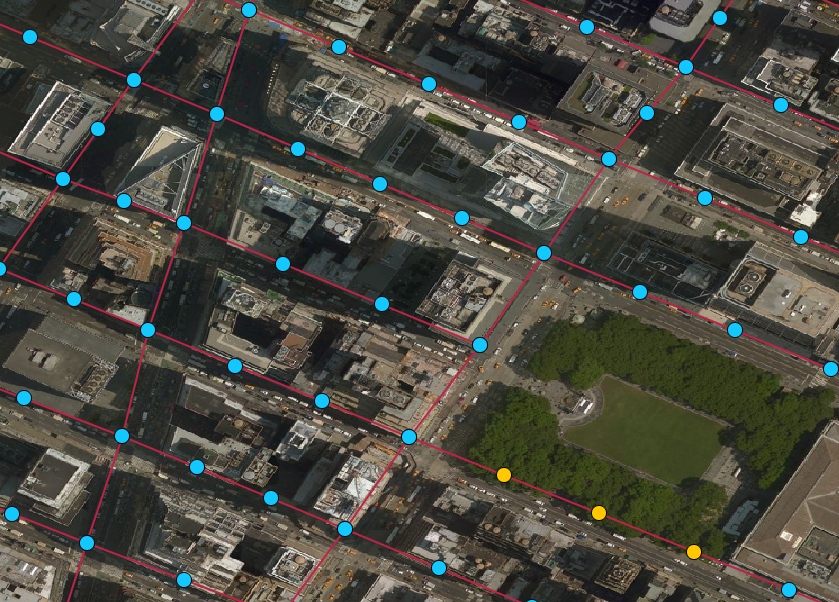
\includegraphics[width=0.8\textwidth]{src/fig/road}
\caption{Portion of a road network graph showing edges (red lines) and vertices
(blue circles) overlayed on top of Manhattan (QGIS 2.18.16, Bing Aerial).
Vertices do not have to be at an intersection (orange circles, lower right).}
\label{fig:road}
\end{figure}

\hi{Paths.}
A path $p=(p_i)_{i\in 1..n}=p_1..p_n$ is a sequence of $n$ vertices
such that any two adjacent vertices are an edge, or $(p_i,p_{i+1})\in \mathcal{E}$ for
$i\in 1..(n-1)$.
A vertex or edge can appear multiple times in a path.
The \emph{path distance} is
$$\sum_{i=1}^{n-1} d(p_i, p_{i+1}).$$
Path $p$ is a \emph{shortest path} only if it minimizes the distance out of all
possible paths from $p_1$ to $p_n$.
Multiple shortest paths are possible.

\hi{Waypoints.}
Waypoints are used to describe points in time as well as space.
A waypoint is a tuple $(\texttt{t},\texttt{v})$, with the
domain of $\texttt{t}$ as $1..H$ and the domain of $\texttt{v}$ as
$\mathcal{V}$. Waypoints can be labeled in a way that will be
discussed later.

\hi{Routes.}
Routes are formed by a sequence of waypoints. A route
$w=(w_i)_{i\in 1..n}=w_1..w_n=(t_1,v_1)..(t_n,v_n)$
is defined as a sequence of $n$ waypoints such that
$t_1..t_n$ is strictly increasing and $v_1..v_n$ is a path.
%In other words it is a binary relation on time and $\mathcal{V}$.
In the spatial dimension, function
$$D(w)=\sum_{i=1}^{n-1}d(\pi_\texttt{v}(w_i),\pi_\texttt{v}(w_{i+1}))$$
gives the \emph{route distance}, analogous to path distance.
% Abandoned: wordy. Projection $\pi_\texttt{v}(w_i)$ returns the vertex component of waypoint $w_i$.
In the time dimension, function
$$\delta(w)=\pi_\texttt{t}(w_n)-\pi_\texttt{t}(w_1)$$
gives the \emph{route duration}.
%The \emph{distance} of $w$ is $D(\pi_\texttt{v}(w))$.
%The \emph{duration} of $w$ is $t_n$.
Given a time $t$,
\begin{align*}
w_{\leq t}=\textrm{sort}(\sigma_{\texttt{t}\leq t}(w))\quad\textrm{and}\quad
w_{>t}=\textrm{sort}(\sigma_{\texttt{t}>t}(w))
\end{align*}
give the \emph{traveled route} denoted $w_{\leq t}$, and the \emph{remaining
route} denoted $w_{>t}$. As the selection operator imposes no ordering on the resulting
set, a $\textrm{sort}(...)$ function is introduced to
sort a set of waypoints by time in ascending order, returning a sequence.
% From now on, any selection or projection on time is assumed to be sorted
% in this manner.
For two adjacent waypoints $w_i$ and~$w_{i+1}$, function
$$\nu(w_i,w_{i+1})=\frac{d(\pi_\texttt{v}(w_i),\pi_\texttt{v}(w_{i+1}))}
{\pi_\texttt{t}(w_{i+1})-\pi_\texttt{t}(w_i)}$$ gives the
\emph{waypoint rate}, or more intuitively the \emph{speed}.
% The unit of speed depends on the units of $d$ and time and do not have to be
% a physical velocity, such as meters per second.
As $d$ only applies to edges, $\nu$ only applies to adjacent waypoints.
Speeds can be bounded above by a value $\nu^\textrm{max}(v_i,v_{i+1})$ on each edge,
for example to describe road speed limits.
%The speed limit can be different
%on different edges, but to simplify the notation, let $\nu_{max}$ denote the limit for any edge.
%Note that duration $t_n$ and distance $D(\pi_\texttt{v}(w))$ are
%convertible through the speeds along each of the edges.

\subsection{Requests and Servers}
\label{ch:1:sec:requests-and-servers}
Now we define the requests and servers.
The basic entity representing a ridesharing participant is the \emph{user}.  A
user is classified as a \emph{request} if it represents a Type~1 or Type~2
customer, or classified as a \emph{server} if it represents a Type~3 or Type~4
vehicle. As only vehicles can move about (P4), only servers are associated with
routes in order to describe the motions. Later, \emph{schedules} describing
pick-up and drop-off events will be defined on the routes.

\hi{User Relation}
A user $u$ is a 5-tuple defined by
${u:=(\texttt{q},\texttt{e},\texttt{l},\texttt{o},\texttt{d})}$.  The
\texttt{q} component corresponds to the user load; the \texttt{e} and
\texttt{l} components correspond to the user early and late times; the
\texttt{o} and \texttt{d} components correspond to the user origin and
destination.
From P1--P4, the domain of \texttt{q} is the non-zero integers; the domain of \texttt{e} is
$1..(H-1)$ and the domain of \texttt{l} is $(u_\texttt{e}+1)..H$; the domains
of \texttt{o} and \texttt{d} are both $\mathcal{V}$.
For a Type 4 vehicle, the destination can be set to a dummy vertex with edge
weight equal to 0 to every other vertex in the road network.

The set of all users forms the 5-ary relation $\mathcal{U}$, called
the \emph{user relation}.
The set
$\mathcal{U}_\texttt{o}=\pi_\texttt{o}(\mathcal{U})$ contains all origins and
$\mathcal{U}_\texttt{d}=\pi_\texttt{d}(\mathcal{U})$ contains all destinations.
From P1, a user can be classified as either a request or a server based on its load.

From now on as a convenience, the notation $d_u$ will be used to denote the distance of the
shortest path from $u_\texttt{o}$ to $u_\texttt{d}$ on graph $\mathcal{G}$, and
the notation $\delta_u$ will be used to denote the shortest travel duration
along $d_u$ using the speed limits $\nu^\textrm{max}$ along the shortest-path edges.

\hi{Requests.}
A request represents a Type 1 or Type 2 customer.
According to P1,
relation $\mathcal{R}\subseteq\mathcal{U}$,
$$\mathcal{R}=\sigma_{\texttt{q}>0}(\mathcal{U}),$$
% Abandoned: $$\mathcal{R}=\{r\in \mathcal{U}\mid r_\texttt{q}>0\},$$
forms the set of all requests by taking users with positive loads. The set
$\mathcal{R}_\texttt{o}=\pi_\texttt{o}(\mathcal{R})$ is the set of all request origins and
$\mathcal{R}_\texttt{d}=\pi_\texttt{d}(\mathcal{R})$ is the set of all request destinations.
%Abandoned: "corresponding" vertices
%Abandoned: Vertex $v$ is a \emph{pickup} if $v\in \mathcal{R}_o$ and it is a
%\emph{dropoff} if $v\in \mathcal{R}_d$.

\hi{Servers.}
Likewise, a server represents a Type 3 or Type 4 vehicle.
From P1, the relation $\mathcal{S}=\mathcal{U}\setminus\mathcal{R}$, or
$$\mathcal{S}=\sigma_{\texttt{q}<0}(\mathcal{U}),$$
% Abandoned: $$\mathcal{S}=\{s\in \mathcal{U}\mid s_\texttt{q}<0\},$$
forms the set of all servers. The set
$\mathcal{S}_\texttt{o}=\pi_\texttt{o}(\mathcal{S})$ is the set of all server origins and
$\mathcal{S}_\texttt{d}=\pi_\texttt{d}(\mathcal{S})$ is the set of all server destinations.
%Abandoned: The vehicle has a speed $\nu(a,b)$ along edge $(a,b)$. For
%simplicity, denote the speed as $\nu$ for all vehicles and all edges.

\hi{Routes and Schedules}
To encode vehicle motions, each server $s\in\mathcal{S}$ is associated with a
route and a schedule.  A server's route is a representation of the corresponding
vehicle's motion through the road network while a server's schedule
encodes the times and locations of customer pick-ups and drop-offs.
The schedule describes the events along the route and not any new motion,
therefore it is a subsequence of the server's route.

\hi{Server Routes.}
Let $w$ be the route for server $s$. As time
advances, the traveled route $w_{\leq t}$ encodes the server's past
motion while the remaining route $w_{>t}$ encodes the future motion.
From P2 and P3, the route is subject to two rules:
\begin{enumerate}
\item[R1.] The time component of the first waypoint equals the server's early time,
  and the time component of the last waypoint is not greater than the server's late time,
  or $\pi_\texttt{t}(w_1)=s_\texttt{e}$ and $\pi_\texttt{t}(w_{|w|})\leq s_\texttt{l}$;
\item[R2.] The vertex components of the first and last waypoints equal the
  server's origin and destination respectively, or
  $\pi_\texttt{v}(w_1)=s_\texttt{o}$ and $\pi_\texttt{v}(w_{|w|})=s_\texttt{d}$.
\end{enumerate}

\hi{Server Schedules.}
A server's schedule
$$b=(b_j)_{j\in 1..m}=(w_{i_j})_{j\in 1..m}=(t_{i_1},v_{i_1})..(t_{i_m},v_{i_m})$$
is a subsequence of the server's route $w$, with $m\leq |w|$ waypoints.
First:
\begin{enumerate}
\item[R3.] The first and last waypoints $b_1$ and $b_m$ equal the first and last
waypoints of $w$, or ${b_1=w_1}$ and ${b_m=w_{|w|}}$.
\end{enumerate}
This rule will help later when defining departure and arrival times.
Second, from P5:
\begin{enumerate}
\item[R4.] For each waypoint $b_j$ for $j\in 2..(m-1)$, the vertex component is either a
request origin or request destination, or $\pi_\texttt{v}(b_j)\in
\mathcal{R}_\texttt{o}\cup\mathcal{R}_\texttt{d}$.
\end{enumerate}
In other words, each entry or exit must occur at a customer origin or destination.

A schedule formalizes the notion of shared travel with other users, as
multiple entries and exits can overlap within the same server route.
At time $t$, the \emph{traveled schedule} denoted $b_{\leq t}$ encodes the past entries and exits and is given by
$\sigma_{\texttt{t}\leq t}(b)$. Likewise, the \emph{remaining schedule} denoted
$b_{>t}$ encodes the future entries and exits and is given by $\sigma_{\texttt{t}>t}(b)$.

\hi{Schedule Labels.}
Each waypoint in schedule $b$ has a set of labels in order to identify which
customers are entering and exiting the vehicle at the waypoint's time and location.
A labeling scheme can be applied to $b$ to determine each of the labels. The
set of all possible labels depends on the locations of the waypoints. Let
$$\mathcal{R}'=\sigma_{\texttt{o}\in\pi_\texttt{v}(b)\lor \texttt{d}\in\pi_\texttt{v}(b)}(\mathcal{R})$$
%Abandoned: $$\mathcal{R}'=\{r\in \mathcal{R}\mid
%     r_\texttt{o}\in\pi_\texttt{v}(b)\vee r_\texttt{d}\in\pi_\texttt{v}(b)\}$$
give the set of requests whose origin or destination is found
in at least one waypoint in $b$. The labeling scheme
\begin{equation*}
L:b\rightarrow \mathbb{P}(\mathcal{R}'\cup\{s\})
\end{equation*}
maps elements of $b$ to elements of the power set of $\mathcal{R}'\cup\{s\}$.
By using the power set $\mathbb{P}$,
a waypoint can have multiple labels, representing the case where multiple customers
enter or exit the vehicle at the waypoint.
The labeling scheme is subject to the following labeling rules:
\begin{enumerate}
\item[R5.] No waypoint can be labeled with $r\in\mathcal{R}'$ if a schedule for another server
already contains waypoints labeled with $r$;
\item[R6.] A waypoint $b_j\in b$ can be labeled with $r$ only if
$\pi_\texttt{v}(b_j)=r_\texttt{o}$ or $\pi_\texttt{v}(b_j)=r_\texttt{d}$;
\item[R7.] If $b_j$ is to be labeled with $r$ and $\pi_\texttt{v}(b_j)=r_\texttt{o}$, then
a second waypoint $b_{j'}$ such that $j'>j$ and
$\pi_\texttt{v}(b_{j'})=r_\texttt{d}$ must also be labeled with $r$;
\item[R8.] The time components of $b_j$ and $b_{j'}$ must be within request $r$'s time window,
formally $r_\texttt{e}\leq \pi_\texttt{t}(b_j)$ and $\pi_\texttt{t}(b_{j'})\leq r_\texttt{l}$;
\item[R9.] The number of waypoints labeled with $r$ must be exactly 0 or 2;
\item[R10.] The first and last waypoints must contain the schedule's server $s$
in their labels, and no other waypoint can be labeled with $s$.
\end{enumerate}
Rules R5--R9 express P5.  Rule R10 can be interpreted to mean that a vehicle
must ``serve itself'' at its own origin and destination.  This last rule
helps to define later concepts.

\hi{Server Relation}
By combining the routes, schedules, and labels into
a set of $(\texttt{s},\texttt{t},\texttt{v},\texttt{L})$ tuples, a
4-ary relation $\mathcal{X}$ can be formed. This relation is called the
\emph{server relation} and as will be shown soon, it is the basis for computing many common ridesharing metrics.
Each tuple associates the waypoint in the \texttt{t} and \texttt{v} components with the server
in the \texttt{s} component, along with the labels in the \texttt{L} component.
% The domain of $\texttt{s}$ is $\mathcal{S}$; the domain of $\texttt{t}$ is
% $1..H$; the domain of $\texttt{v}$ is $\mathcal{V}$; the domain of $\texttt{L}$
% is the power set $\mathbb{P}(\mathcal{U})$.

A server's route can be recovered by extracting \texttt{t} and \texttt{v}
components and sorting by time, or formally for a given server $s$, its route
is given by
$$W(\mathcal{X},s)=\textrm{sort}(\pi_{\texttt{t},\texttt{v}}(\sigma_{\texttt{s}=s}(\mathcal{X}))).$$
Similarly, a server's schedule can be recovered by
extracting only those waypoints that are labeled, formally
$$B(\mathcal{X},s)=\textrm{sort}(\pi_{\texttt{t},\texttt{v}}(\sigma_{\texttt{s}=s\land |\texttt{L}|>0}(\mathcal{X}))).$$

The server relation can be used to define the remaining physical concepts, P6 and P7.

\hi{Request Status.}
Given a request $r$, the function
\begin{equation}
\label{eq:status}
\textrm{status}(\mathcal{X},r,t)=|\sigma_{\texttt{t}\leq t\land
r\in\texttt{L}}(\mathcal{X})|
\end{equation}
gives the count of the tuples labeled with $r$
before or on a given time. From the labeling rules, the count can be only 0, 1,
or 2. See that these counts correspond to request waiting, in-transit, and arrived states
from P7, respectively.

Given a server $s$, knowing the in-transit requests for $s$ can be useful for
pricing and other rider-related
metrics. %~\cite{DBLP:conf/sigmod/ChengX017,DBLP:conf/dexa/ShiLZG17,DBLP:conf/ijcai/SantosX13}.
These requests can be easily found by
$$\mathcal{Q}(\mathcal{X},s,t)=\{r\in\mathcal{R}\mid\textrm{status}(\mathcal{X},r,t)=1
\land\pi_\texttt{s}(\sigma_{r\in\texttt{L}}(\mathcal{X}))=s\}.$$

\hi{Load Burden.}
The \emph{load burden} on $s$ can be computed using the in-transit requests by
\begin{equation}
\label{eq:load}
Q(\mathcal{X},s,t)=\sum_{r\in\mathcal{Q}(\mathcal{X},s,t)}r_\texttt{q}.
\end{equation}
From P6, server routes are subject to the additional rule:
\begin{enumerate}
\item[R11.] $Q(\mathcal{X},s,t)\leq -s_\texttt{q}$ must be true for all $s$ and $t$.
\end{enumerate}

\subsection{Ridesharing Metrics}
\label{ch:1:sec:ridesharing-metrics}
As a benefit from using relations, a variety of metrics can now be measured by
simple operations on $\mathcal{U}$ and $\mathcal{X}$.  The following lists
common metrics found in existing ridesharing studies, but others may be possible.

\hi{Assignments.}
Server $s$ is said to be \emph{assigned to} request $r$ at time $t$ only if
$\textrm{status}(\mathcal{X},r,t)=2$. That is, the request's status is arrived at time $t$.
The set of $(s,r)$ pairs
where this property is true is called the set of \emph{assignments}, formally
\begin{equation}
\label{eq:assignments}
\textit{assignments }A(\mathcal{X},t)=
\{(s,r)\in\mathcal{S}\times \mathcal{R} \mid \textrm{status}(\mathcal{X},r,t)=2\}.
\end{equation}
Using the assignments,
\begin{align}
\label{eq:assigned-requests}
\textit{assigned requests }R^\textrm{ok}(\mathcal{X},t)&=\pi_\texttt{r}(A(\mathcal{X},t))\textrm{, and}\\
\label{eq:unassigned-requests}
\textit{unassigned requests }R^\textrm{ko}(\mathcal{X},t)&=\mathcal{R}\setminus\mathcal{R}^\textrm{ok}(\mathcal{X},t).
\end{align}
The server assigned to $r$ can be obtained with
\begin{equation}
S(\mathcal{X},r,t)=\{s\in\mathcal{S}\mid\textrm{status}(\mathcal{X},r,t)=2\},
\end{equation}
guaranteed to return only one server due to R5.
Likewise, the set of requests assigned to $s$ can be obtained with
\begin{equation}
\label{eq:R(X,s,t)}
R(\mathcal{X},s,t)=\{r\in\mathcal{R}\mid\textrm{status}(\mathcal{X},r,t)=2\}.
\end{equation}

\hi{Service rate.}
The \emph{service rate} is the number of assigned requests over the number of all requests, or
\begin{equation}
\label{eq:service-rate}
\textit{service rate }\mu(\mathcal{X},t)=\frac{|R^\textrm{ok}(\mathcal{X},t)|}{|\mathcal{R}|}.
\end{equation}

\hi{Distances.}
The \emph{base distance} is the sum of the shortest-path distances for all users, or
\begin{equation}
\label{eq:base-distance}
\textit{base distance }D^\textrm{base}(\mathcal{U})=\sum_{u\in U}d_u.
\end{equation}
The \emph{travel distance} for one server $s$ is the distance of its route,
$D(W(\mathcal{X},s))$,
and the \emph{travel duration} can be found with
$\delta(W(\mathcal{X},s))$.

For a server with route $w$, travel distance $D(w)$ can be partitioned into
\emph{cruising distance} $D_0(w)$ and
\emph{service distance} $D_1(w)$.
The cruising distance sums the distance along portions where the load burden is zero.
The service distance sums the distance along portions of $w$ where the
load burden is non-zero.
Formally, partition $w$ into a set of substrings $\Omega(w)$ such that each waypoint
in $w$ is a member of exactly one substring and that for all substrings $\omega\in \Omega$,
\begin{align}
\label{eq:slack}\textrm{either }Q(\mathcal{X},s,t)&=0\textrm{ is true for all }t\in \pi_\texttt{t}(\omega),\\
\label{eq:block}\textrm{or }Q(\mathcal{X},s,t)&>0\textrm{ is true for all }t\in \pi_\texttt{t}(\omega).
\end{align}
%Observe that Eqs.~\ref{eq:slack}~and~\ref{eq:block}
%formalize concepts similar to the intuitive
%\emph{slack periods} and \emph{schedule blocks} in~\cite{jaw:1986}.
The equations can be used to partition $\Omega(w)$ into two subsets,
\begin{align*}
\Omega_0(w)&=\{\omega\in \Omega(w)\mid \omega\textrm{ satisfies Eq.~\ref{eq:slack}}\}\textrm{ and }\\
\Omega_1(w)&=\{\omega\in \Omega(w)\mid \omega\textrm{ satisfies Eq.~\ref{eq:block}}\}.
\end{align*}
The distances of each of the substrings in each subset can be summed
to get
$$D_0(w)=\sum_{\omega\in \Omega_0(w)} D(\omega)\quad\textrm{and}\quad
  D_1(w)=\sum_{\omega\in \Omega_1(w)} D(\omega).$$
These distances are written as
\begin{align}
\label{eq:cruising-distance}
\textit{cruising distance }D^\textrm{cruise} (\mathcal{X},s)&=D_0(W(\mathcal{X},s)),\textrm{ and}\\
\label{eq:service-distance}
\textit{service distance } D^\textrm{service}(\mathcal{X},s)&=D_1(W(\mathcal{X},s)).
\end{align}

\hi{Detours and Delays.}
In physical terms, the \emph{detour route} for a customer is the portion of a vehicle's
route between when it visits the customer's origin and destination. Formally, let
%\item $d_r$ be the distance of the shortest path from $r_\texttt{o}$ to $r_\texttt{d}$;
$w=W(\mathcal{X},S(\mathcal{X},r,H))$ be the route of the server assigned to $r$.
The detour route $\Delta W(\mathcal{X},r)$ is an $m$-length substring of $w$ given by
$\Delta W(\mathcal{X},r)=w_{1+k}..w_{m+k}$ such that for some $k$,
\begin{itemize}
\item $\Delta W(\mathcal{X},r)$ begins at $r_\texttt{o}$, or $\pi_\texttt{v}(w_{1+k})=r_\texttt{o}$,
\item $\Delta W(\mathcal{X},r)$ ends at $r_\texttt{d}$, or $\pi_\texttt{v}(w_{m+k})=r_\texttt{d}$, and
\item the first and last waypoints of $\Delta W(\mathcal{X},r)$ are labeled with $r$, or $r\in\pi_\texttt{L}(w_{1+k})\cap\pi_\texttt{L}(w_{m+k})$.
\end{itemize}
Observe that due to the labeling rules, only one value of $k$ can satisfy these
conditions. The first and last waypoints $w_{1+k}$ and $w_{m+k}$ can be found by
the equations on users,
\begin{align}
\label{eq:pickup}
\textrm{pickup}(\mathcal{X},u)&=\pi_{\texttt{t},\texttt{v}}(\sigma_{\texttt{v}=u_\texttt{o}\land u\in\texttt{L}}(\mathcal{X}))\textrm{, and}\\
\label{eq:dropoff}
\textrm{dropoff}(\mathcal{X},u)&=\pi_{\texttt{t},\texttt{v}}(\sigma_{\texttt{v}=u_\texttt{d}\land u\in\texttt{L}}(\mathcal{X})),
\end{align}
by substituting $r$ for $u$.
Note that if a server is substituted for $u$, these equations give the start and
end waypoints of the server's route due to R3 and R10.
These two equations can also be used to give two times for
any user,
\begin{align}
\label{eq:departure-time}
\textit{departure time }t^\textrm{depart}(\mathcal{X},u)&=\pi_\texttt{t}(\textrm{pickup}(\mathcal{X},u))\textrm{, and}\\
\label{eq:arrival-time}
\textit{arrival time }t^\textrm{arrive}(\mathcal{X},u)&=\pi_\texttt{t}(\textrm{dropoff}(\mathcal{X},u)).
\end{align}
In the real world, the time until a vehicle picks up a customer can be of interest.
This \emph{pick-up delay} can be found with
\begin{equation}
\label{eq:pick-up delay}
\textit{pick-up delay }\delta^\textrm{pickup}(\mathcal{X},r)=\pi_\texttt{t}(\textrm{pickup}(\mathcal{X},r))-r_\texttt{e}.
\end{equation}

The detour route $\Delta W(\mathcal{X},r)$ can only apply to assigned requests. If
a detour route exists, then
the \emph{transit} distance and duration are
\begin{align}
\label{eq:transit-distance}
\textit{transit distance }D^\textrm{transit}(\mathcal{X},r)&=D(\Delta W(\mathcal{X},r))\textrm{, and}\\
\label{eq:transit-duration}
\textit{transit duration }\delta^\textrm{transit}(\mathcal{X},r)&=\delta(\Delta W(\mathcal{X},r)).
\end{align}
Similarly, the \emph{detour} distance and duration are
\begin{align}
\label{eq:detour-distance}
\textit{detour distance }D^\textrm{detour}(\mathcal{X},r)&=D^\textrm{transit}(\mathcal{X},r)-d_r\textrm{, and}\\
\label{eq:detour-duration}
\textit{detour duration }\delta^\textrm{detour}(\mathcal{X},r)&=\delta^\textrm{transit}(\mathcal{X},r)-\delta_r.
\end{align}
Finally, the \emph{travel duration} is the sum of the pick-up and transit durations,
\begin{equation}
\label{eq:travel-duration}
\textit{travel duration }\delta^\textrm{travel}(\mathcal{X},r)=\delta^\textrm{pickup}(\mathcal{X},r)+\delta^\textrm{transit}(\mathcal{X},r)
=\pi_\texttt{t}(\textrm{dropoff}(\mathcal{X},r))-r_\texttt{e}.
\end{equation}

\hi{Utilization.}
The percentage of servers that are assigned to at least one request is given by
\begin{equation}
\label{eq:server-utilization}
\textit{server utilization }\rho^\textrm{server}(\mathcal{X})=\frac{|\pi_\texttt{s}(\mathcal{A}(\mathcal{X}))|}{|\mathcal{S}|}.
\end{equation}
The distance utilization is
\begin{equation}
\label{eq:distance-utilization}
\textit{distance utilization }\rho^\textrm{distance}(\mathcal{X})=
\frac{\sum_{s\in\mathcal{S}}D^\textrm{service}(\mathcal{X},s)}
{\sum_{s\in\mathcal{S}}D(\mathcal{X},s)}.
\end{equation}

\section{Ridesharing Data Model}
\label{ch:1:sec:ridesharing-data-model}
The simple constraints allowed by the SQL standard\footnote{ISO/IEC 9075}
(\texttt{CHECK}, \texttt{UNIQUE}, \texttt{NOT NULL}, \texttt{FOREIGN KEY}) are
unable to express the complex ridesharing properties
(\S\ref{ch:1:sec:ridesharing-systems}, P1--P7) and rules
(\S\ref{ch:1:sec:ridesharing-formulation}, R1--R11), and consequently a direct
``translation'' of the ridesharing relations into SQL is not possible without
either making code extensions to SQL or reorganizing the relational ridesharing
model.

The following schema can be implemented entirely in standard SQL without any
code extensions while staying faithful to the model.  In this schema,
\textit{tables} capture the descriptive elements of the model and
\textit{views} express the analytical measures.  Tables are further organized
into \emph{property}, \emph{solution}, and \emph{constraint} tables.  Property
tables store the road network $\mathcal{G}$ (\S\ref{ch:1:sec:setting}) and the user
relation $\mathcal{U}$ (\S\ref{ch:1:sec:requests-and-servers}).  Solution tables
store the server relation $\mathcal{X}$ (\S\ref{ch:1:sec:requests-and-servers}).
Constraint tables store copies of data from other tables for validation
purposes.  The views are mostly defined on the constraint tables.

Diagrams of the SQL tables are included in this section. In the diagrams,
primary keys are indicated in italics. Elsewhere, column names are
distinguished by \textsf{sans serif} script.  Parentheses are used to logically
group together columns.  A parent table next to a group of columns indicates
foreign key. In SQL, foreign keys must reference their values from the primary
key of the parent table. Many of the table diagrams contain duplicate columns
(for example, \textsf{sid} shows up three times in Table W).  These duplicates
are included for illustrating the foreign key relationships, but in practice
the duplicates are implemented as single columns participating in multiple
foreign keys.

\subsection{Table V and E (Road Network Tables)}
Each vertex $v\in\mathcal{V}$ is stored in Table V along with its coordinates
$V(v)$ while each edge $(a,b)\in\mathcal{E}$ is stored in Table E along with
its weight $d(a,b)$ and speed limit $\nu^\textrm{max}(a,b)$.  Table V thus has
three columns, storing $v$ in primary key column \textsf{v} ([[P1]]) and its
coordinates in column \textsf{lng} and \textsf{lat}.  Likewise, Table E has
four columns, storing $a$ and $b$ in column \textsf{v1} and \textsf{v2},
$d(a,b)$ in column \textsf{dd}, and $\nu^\textrm{max}(a,b)$ in column
\textsf{nu}.  The four columns together form the primary key ([[P2]]) in order
to be referenced by later tables.  Foreign keys on \textsf{v1} ([[F1]]) and
\textsf{v2} ([[F2]]) referencing Table V validate that $a$ and $b$ are actual
vertices.
\begin{table}[h]
\centering
\small
\begin{tabular}{|c|l|}
\hline
\rowcolor{TableTitle}
\multicolumn{2}{|c|}{Table V (Vertices)}\\
\hline
\rowcolor{TableHeader}
Column & Description\\
\hline
\textit{v} & Vertex $v\in\mathcal{V}$\\
\hline
lng & \multirow{2}{*}{Vertex coordinate $V(v)$}\\
lat & \\
\hline
\end{tabular}
\begin{tabular}{|c|c|l|}
\hline
\rowcolor{TableTitle}
\multicolumn{3}{|c|}{Table E (Edges)}\\
\hline
\rowcolor{TableHeader}
Column & Parent & Description\\
\hline
\textit{v1} & Table V & \multirow{2}{*}{Edge $(a, b)\in\mathcal{E}$} \\
\cline{2-2}
\textit{v2} & Table V & \\
\hline
\textit{dd} & & Weight $d(a,b)$\\
\hline
\textit{nu} & & Max. speed $\nu^\textrm{max}(a,b)$\\
\hline
\end{tabular}
\end{table}

\subsection{Table UQ, UE, UL, UO, UD, and UB (User Tables)}
To allow other tables to reference specific user components, the user relation
is partitioned into five 2-column tables, UQ, UE, UL, UO, and UD, by taking
projections on the respective \texttt{q}, \texttt{e}, \texttt{l}, \texttt{o},
and \texttt{d} components. Each row is a key-value pair, storing a unique
\textsf{uid} for user identification as the key alongside the component value,
and each row is also its own primary key.  A sixth table UB is introduced to
store base costs for computing $D^\textrm{base}$ and $\rho^\textrm{distance}$
(\S\ref{ch:1:sec:ridesharing-metrics}).  Table UO and UD can be referenced to Table
V to validate against property P2 and rule P4.
\begin{table}[h]
\centering
\small
\begin{tabular}{|c|c|l|}
\hline
\rowcolor{TableTitle}
\multicolumn{3}{|c|}{User Tables}\\
\hline
\rowcolor{TableHeader}
Table & Columns & Description \\
\hline
UQ & \textit{uid}, \textit{val} & User load $u_\texttt{q}$ \\
UE & \textit{uid}, \textit{val} & User early time $u_\texttt{e}$ \\
UL & \textit{uid}, \textit{val} & User late time $u_\texttt{l}$ \\
UO & \textit{uid}, \textit{val} & User origin $u_\texttt{o}$ \\
UD & \textit{uid}, \textit{val} & User destination $u_\texttt{d}$ \\
UB & \textit{uid}, \textit{val} & User base cost $d_u$ \\
\hline
\end{tabular}
\end{table}

\subsection{Table W (Routes Table)}
Table W has eight columns, \textsf{sid}, \textsf{se}, \textsf{t1}, \textsf{v1},
\textsf{t2}, \textsf{v2}, \textsf{dd}, and \textsf{nu}.  The \texttt{s},
\texttt{t}, and \texttt{v} components of $\mathcal{X}$ are stored in the
(\textsf{sid}, \textsf{t2}, \textsf{v2}) columns.  By definition, the sequence
of vertices in a route must form a path and the speed of adjacent waypoints
cannot exceed the limit $\nu^\textrm{max}$.  To enforce these rules, the
\emph{predecessor} waypoint is stored in the (\textsf{sid}, \textsf{t1},
\textsf{v1}) columns.  The (\textsf{v1}, \textsf{v2}) columns can thus identify
an edge. Columns \textsf{dd} and \textsf{nu} are added to store the weight and
speed limit on the edge, and (\textsf{v1}, \textsf{v2}, \textsf{dd},
\textsf{nu}) is referenced by foreign key to Table E ([[F19]]) to validate the
values. A row-level \texttt{CHECK} constraint ([[C56]]) validates that the
speed $\textsf{dd}/(\textsf{t2}-\textsf{t1})$ is not greater than the maximum
free-flow speed, \textsf{nu}.
\begin{table}[h]
\centering
\small
\begin{tabular}{|c|c|l|}
\hline
\rowcolor{TableTitle}
\multicolumn{3}{|c|}{Table W (Routes)} \\
\hline
\rowcolor{TableHeader}
Col. & Parent & Description \\
\hline
\textit{sid} & Table S & Identification for server $s\in\mathcal{S}$ \\
\hline
sid & \multirow{2}{*}{Table UE} & \multirow{2}{*}{Server early time $s_\texttt{e}$} \\
se & & \\
\hline
sid & \multirow{3}{*}{Table W} & \multirow{3}{*}{Predecessor waypoint $w_{i-1}$} \\
t1 & & \\
v1 & & \\
\hline
\textit{t2} & & \multirow{2}{*}{Waypoint $w_i$} \\
\textit{v2} & & \\
\hline
v1 & \multirow{4}{*}{Table E} & \multirow{4}{*}{Properties of edge $(\pi_\texttt{v}(w_{i-1}),\pi_\texttt{v}(w_i))$} \\
v2 & & \\
dd & & \\
nu & & \\
\hline
\end{tabular}
\end{table}
The below items are easily implemented in SQL and establish that each
(\textsf{sid}, \textsf{t1}, \textsf{v1}) is indeed the predecessor to
(\textsf{sid}, \textsf{t2}, \textsf{v2}) in the same row:
\begin{enumerate}
\item The predecessor (\textsf{sid}, \textsf{t1}, \textsf{v1}) must reference
an existing waypoint (\textsf{sid}, \textsf{t2}, \textsf{v2}) from the table
([[F20]]);
\item Out of all rows, (\textsf{sid}, \textsf{t1}) must be unique and
(\textsf{sid}, \textsf{t2}) must be unique ([[C54]], [[C55]]);
\item Column \textsf{t2} and \textsf{v2} cannot be null ([[C52]], [[C53]]);
\item Unless \textsf{t2} is equal to the server's early time, \textsf{t1}
cannot be null and it must be less than \textsf{t2}, otherwise \textsf{t1},
\textsf{v1}, \textsf{dd}, and \textsf{nu} must all be null ([[C56]]).
\end{enumerate}
The (\textsf{sid}, \textsf{t2}, \textsf{v2}) columns are the primary key
([[P11]]) in order to allow the self-referencing foreign key in the first item.
The last item handles the case where the first waypoint in a server's route has
no predecessor. Only in this case are \textsf{t1}, \textsf{v1}, \textsf{dd},
and \textsf{nu} are allowed to be null.  From rule R1, the first waypoint is
detected by checking if \textsf{t2} is equal to the server's early time, stored
in column \textsf{se}. The (\textsf{sid}, \textsf{se}) columns are referenced
to UE to validate the early time ([[F18]]).

\subsection{Table PD (Labels Table)}
Table PD (for ``pick-ups and drop-offs'') contains four columns, \textsf{sid},
\textsf{t2}, \textsf{v2}, and \textsf{rid}.  The (\textsf{sid}, \textsf{t2},
\textsf{v2}) columns reference Table W ([[F23]]), and the \textsf{rid} column
indicates the label on that waypoint.  Each row is its own primary key
([[P12]]) in order to be referenced by the CPD constraint table.  A waypoint
can have multiple labels simply by listing the waypoint multiple times with
different values of \textsf{rid}.
\begin{table}[h]
\centering
\small
\begin{tabular}{|c|c|l|}
\hline
\rowcolor{TableTitle}
\multicolumn{3}{|c|}{Table PD (Pick-up and Drop-off Labels)}\\
\hline
\rowcolor{TableHeader}
Col. & Parent & Description \\
\hline
\textit{sid} & \multirow{3}{*}{Table W} & \multirow{3}{*}{Waypoint $w_i$ (schedule element $b_j$)} \\
\textit{t2} & & \\
\textit{v2} & & \\
\hline
\textit{rid} & Table R & Identification for request $r\in\mathcal{R}$ \\
\hline
\end{tabular}
\end{table}

\subsection{Table S and R (User Constraint Tables)}
Table S and Table R enforce the remaining user constraints.  Both tables have
six columns, one for each of \textsf{uq}, \textsf{ue}, \textsf{ul},
\textsf{uo}, \textsf{ud}, and \textsf{ub}, to store user data. A seventh column
stores the user identifier as the primary key. The identifier is stored in the
\textsf{sid} column for Table S and the \textsf{rid} column for Table R.  Each
(\textsf{sid}, column) or (\textsf{rid}, column) pair references the
corresponding user property table, for example (\textsf{sid}, \textsf{uq})
references Table UQ.
% An application must populate S and R for the \textsf{sid} and \textsf{rid} foreign keys in W and PD.

Properties P1 and P3 that could not be enforced in the user tables are now
enforced through simple constraints on S and R.  A \texttt{CHECK} constraint
validates that \textsf{uq} is less than 0 in Table S ([[C40]]), and another
\texttt{CHECK} constraint validates it is greater than 0 in Table R ([[C48]]),
corresponding to servers and requests (property P1). Likewise, a \texttt{CHECK}
constraint validates that \textsf{ue} is less than \textsf{ul} ([[C41]],
[[C49]]) (property P3). None of the columns can be null to prevent incomplete
users.
\begin{table}[h]
\centering
\small
\begin{tabular}{|c|l|}
\hline
\rowcolor{TableTitle}
\multicolumn{2}{|c|}{User Constraint Tables}\\
\hline
\rowcolor{TableHeader}
Table & Columns \\
\hline
Table S & \textit{sid}, sq, se, sl, so, sd, sb \\
Table R & \textit{rid}, rq, re, rl, ro, rd, rb \\
\hline
\end{tabular}
\end{table}

\subsection{Table CW (Route Endpoint Constraints Table)}
Table CW stores the start and end waypoints of each server route.  The table
has nine columns, \textsf{sid}, \textsf{se}, \textsf{sl}, \textsf{so},
\textsf{sd}, \textsf{ts}, \textsf{vs}, \textsf{te}, and \textsf{ve}.  The start
waypoint is stored in (\textsf{sid}, \textsf{ts}, \textsf{vs}) and the end
waypoint is stored in (\textsf{sid}, \textsf{te}, \textsf{ve}). Both of these
groups reference the (\textsf{sid}, \textsf{t2}, \textsf{v2}) columns in Table
W ([[F29]], [[F30]]).  The \textsf{sid} column is set to be \texttt{UNIQUE}
([[C70]]) to prevent a server from being listed multiple times and having
``multiple'' start and end waypoints.  Rule R1 is enforced by adding the
server's early and late times into columns \textsf{se} and \textsf{sl},
referencing (\textsf{sid}, \textsf{se}) to UE ([[F25]]) and (\textsf{sid},
\textsf{sl}) to UL ([[F26]]).  A \texttt{CHECK} constraint validates the start
time \textsf{ts} equals \textsf{se} ([[C71]]) and another one validates the end
time \textsf{te} is not beyond \textsf{sl} ([[C72]]).  Rule 2 is enforced by
adding the server's origin and destination into columns \textsf{so} and
\textsf{sd}, referencing (\textsf{sid}, \textsf{so}) to UO ([[F27]]) and
(\textsf{sid}, \textsf{sd}) to UD ([[F28]]).  Likewise, constraint [[C71]]
validates the start location \textsf{vs} equals \textsf{so} and [[C72]]
validates the end location \textsf{ve} equals \textsf{sd}.
\begin{table}[h]
\centering
\small
\begin{tabular}{|c|c|l|}
\hline
\rowcolor{TableTitle}
\multicolumn{3}{|c|}{Table CW (Route Endpoint Constraints)}\\
\hline
\rowcolor{TableHeader}
Col. & Parent & Description\\
\hline
sid & \multirow{2}{*}{Table UE} & \multirow{2}{*}{Server early time $s_\texttt{e}$} \\
se & & \\
\hline
sid & \multirow{2}{*}{Table UL} & \multirow{2}{*}{Server late time $s_\texttt{l}$} \\
sl & & \\
\hline
sid & \multirow{2}{*}{Table UO} & \multirow{2}{*}{Server origin $s_\texttt{o}$} \\
so & &\\
\hline
sid & \multirow{2}{*}{Table UD} & \multirow{2}{*}{Server destination $s_\texttt{d}$} \\
sd & & \\
\hline
\textit{sid} & \multirow{3}{*}{Table W} & \multirow{3}{*}{Server $\textrm{pickup}(\mathcal{X},s)$}\\
\textit{ts} & & \\
vs & & \\
\hline
sid & \multirow{3}{*}{Table W} & \multirow{3}{*}{Server $\textrm{dropoff}(\mathcal{X},s)$}\\
\textit{te} & & \\
ve & & \\
\hline
\end{tabular}
\end{table}

\subsection{Table CPD (Label Constraints Table)}
Table CPD enforces the pick-up and drop-off rules R5--R9. It contains twelve
columns, \textsf{sid}, \textsf{ts}, \textsf{te}, \textsf{tp}, \textsf{vp},
\textsf{td}, \textsf{vd}, \textsf{rid}, \textsf{re}, \textsf{rl}, \textsf{ro},
and \textsf{rd}.  The (\textsf{sid}, \textsf{tp}, \textsf{vp}, \textsf{rid})
and (\textsf{sid}, \textsf{td}, \textsf{vd}, \textsf{rid}) groups reference
rows in Table PD ([[F34]], [[F35]]) and represent pick-up and drop-off
waypoints, respectively.  Rules R5 and R9 are enforced by setting \textsf{rid}
to \texttt{UNIQUE} ([[C86]]), in other words any request identified in
\textsf{rid} has only one pick-up and drop-off pair.  Rule R6 is enforced by
adding columns for the request origin \textsf{ro} and destination \textsf{rd}
and validating that pick-up vertex \textsf{vp} equals \textsf{ro} ([[C89]]) and
drop-off vertex \textsf{vd} equals \textsf{rd} ([[C90]]). The (\textsf{rid},
\textsf{ro}) columns are referenced to UO ([[F38]]) and (\textsf{rid},
\textsf{rd}) are referenced to UD ([[F39]]).  Rules R7 and R8 are enforced by
simple \texttt{CHECK} constraints. Both \textsf{tp} and \textsf{td} are
validated to be between request early time \textsf{re} and late time
\textsf{rl} ([[C89]], [[C90]]). The (\textsf{rid}, \textsf{re}) and
(\textsf{rid}, \textsf{rl}) columns are added and referenced to UE and UL
([[F36]], [[F37]]) for this purpose.

So far, nothing prevents \textsf{tp} and \textsf{td} from falling outside the
server's start and end times. These times are thus added into (\textsf{sid},
\textsf{ts}, \textsf{te}) columns, referenced to Table CW ([[F33]]).  Then,
\texttt{CHECK} constraints can validate that \textsf{tp} and \textsf{td} are
within the start time \textsf{ts} and the end time \textsf{te} ([[C87]],
[[C88]]).
\begin{table}[t]
\centering
\small
\begin{tabular}{|c|c|l|}
\hline
\rowcolor{TableTitle}
\multicolumn{3}{|c|}{Table CPD (Pick-up and Drop-off Constraints)}\\
\hline
\rowcolor{TableHeader}
Col. & Parent & Description \\
\hline
sid & \multirow{3}{*}{Table CW} & \multirow{3}{48mm}{Server start and end times $\pi_\texttt{t}(\textrm{pickup}(\mathcal{X},s))$, $\pi_\texttt{t}(\textrm{dropoff}(\mathcal{X},s))$} \\
ts & & \\
te & & \\
\hline
\textit{sid} & \multirow{4}{*}{Table PD} & \multirow{4}{*}{Request $\textrm{pickup}(\mathcal{X},r)$} \\
\textit{tp} & & \\
vp & & \\
rid & & \\
\hline
sid & \multirow{4}{*}{Table PD} & \multirow{4}{*}{Request $\textrm{dropoff}(\mathcal{X},r)$} \\
\textit{td} & & \\
vd & & \\
\textit{rid} & & \\
\hline
rid & \multirow{2}{*}{Table UE} & \multirow{2}{*}{Request early time $r_\texttt{e}$} \\
re & & \\
\hline
rid & \multirow{2}{*}{Table UL} & \multirow{2}{*}{Request late time $r_\texttt{l}$} \\
rl & & \\
\hline
rid & \multirow{2}{*}{Table UO} & \multirow{2}{*}{Request origin $r_\texttt{o}$} \\
ro & & \\
\hline
rid & \multirow{2}{*}{Table UD} & \multirow{2}{*}{Request destination $r_\texttt{d}$} \\
rd & & \\
\hline
\end{tabular}
\end{table}

\subsection{Table CQ (Load Constraints Table)}
Table CQ enforces the load rule R11. It has fourteen columns, \textsf{sid},
\textsf{sq}, \textsf{se}, \textsf{t1}, \textsf{t2}, \textsf{v2}, \textsf{q1},
\textsf{q2}, \textsf{rid}, \textsf{rq}, \textsf{tp}, \textsf{td}, \textsf{o1},
and \textsf{o2}.  From Eq.~\ref{eq:load}, the load burden only changes at the
times of waypoints labeled with a request. It increases when a waypoint
corresponds to a customer pick-up and decreases when the waypoint corresponds
to a customer drop-off. Each load-changing waypoint is stored in (\textsf{sid},
\textsf{t2}, \textsf{v2}, \textsf{rid}) and referenced to PD ([[F46]]).  To
determine if the waypoint is a customer pick-up or drop-off, the pick-up and
drop-off times for \textsf{rid} are stored in (\textsf{sid}, \textsf{tp},
\textsf{td}, \textsf{rid}) and referenced to CPD ([[F47]]).  If
$\textsf{t2}=\textsf{tp}$, then the waypoint represents a pick-up, otherwise it
represents a drop-off. The load of the server and request are stored in
(\textsf{sid}, \textsf{sq}) and (\textsf{rid}, \textsf{rq}), referenced to UQ
([[F44]], [[F45]]).

To validate if the load burden is always within a server's capacity, CQ must
keep track of every load change. It does so by storing the \emph{predecessor}
load in columns (\textsf{sid}, \textsf{t1}, \textsf{q1}, \textsf{o1}) next to
the current load in columns (\textsf{sid}, \textsf{t2}, \textsf{q2},
\textsf{o2}).  If the waypoint in the row is a pick-up, CQ validates that
$\textsf{q1}+\textsf{rq}=\textsf{q2}$, otherwise that
$\textsf{q1}-\textsf{rq}=\textsf{q2}$ ([[C98]]). As repetitive load changes can
occur at a single waypoint due to multiple pick-ups and drop-offs, the
\textsf{o1} and \textsf{o2} columns are introduced to store a unique
\emph{order number}. This number increments by 1 for each pick-up or drop-off
per server and can be handled by the application. Similar rules for
establishing predecessor waypoints in Table W can be used to establish
predecessor loads in CQ.  Subsequently, (\textsf{sid}, \textsf{t2},
\textsf{q2}, \textsf{o2}) is set to be the primary key ([[P15]]) in order to
allow a self-referencing foreign key on (\textsf{sid}, \textsf{t1},
\textsf{q1}, \textsf{o1}) ([[F42]]), and the server early time is stored in
(\textsf{sid}, \textsf{se}) and referenced to UE ([[F43]]) in order to detect
the first load change.
\begin{table}[t]
\centering
\small
\begin{tabular}{|c|c|l|}
\hline
\rowcolor{TableTitle}
\multicolumn{3}{|c|}{Table CQ (Load Constraints)}\\
\hline
\rowcolor{TableHeader}
Col. & Parent & Description \\
\hline
sid & \multirow{2}{*}{Table UQ} & \multirow{2}{*}{Server load $s_q$} \\
sq & & \\
\hline
sid & \multirow{2}{*}{Table UE} & \multirow{2}{*}{Server early time $s_e$} \\
se & & \\
\hline
sid & \multirow{4}{*}{Table CQ} & \multirow{4}{48mm}{Load burden $\mathcal{Q}(\mathcal{X},s,\textrm{t1})$ up to order o1} \\
t1 & & \\
q1 & & \\
o1 & & \\
\hline
\textit{sid}& & \multirow{3}{48mm}{Load burden $\mathcal{Q}(\mathcal{X},s,\textrm{t2})$ up to order o2} \\
\textit{t2} & & \\
\textit{q2} & & \\
\textit{o2} & & \\
\hline
sid & \multirow{4}{*}{Table PD} & \multirow{4}{48mm}{Request pick-up or delivery waypoint} \\
t2 & & \\
v2 & & \\
rid& & \\
\hline
sid & \multirow{4}{*}{Table CPD} & \multirow{4}{48mm}{Request pick-up and delivery times $\pi_\texttt{t}(\textrm{pickup}(\mathcal{X},r))$, $\pi_\texttt{t}(\textrm{dropoff}(\mathcal{X},r))$} \\
tp & & \\
td & & \\
rid& & \\
\hline
rid & \multirow{2}{*}{Table UQ} & \multirow{2}{*}{Request load $r_q$} \\
rq & & \\
\hline
\end{tabular}
\end{table}

\section{About Literate Programming}
Jargo is developed using the
Noweb\footnote{\url{https://www.cs.tufts.edu/~nr/noweb/}} literate
programming\footnote{\url{http://literateprogramming.com/}} tool.  The files in
the \texttt{src} directory are the source files for both the documentation and
the Java code. See the \texttt{Makefile} for build details.
